\chapter{Oil History}

Petroleum is a commodity which its price follows the law of supply-demand. However, as one of the important strategic materials, there are many factors affecting international oil prices. 
Although supply and demand are the basic determinants, it was also largely influenced by the international economy, political, diplomatic, and military influences, as well as the speculation of the hot money around the world. These influencing factors have effect on short-term oil prices, therefore these long and short term fluctuations in oil prices make it difficult to predict. In this chapter, we will follow the Fig \ref{oilPrice} and briefly introduce the oil price history and the factors affecting it.

\begin{figure}[h]
    \centering
    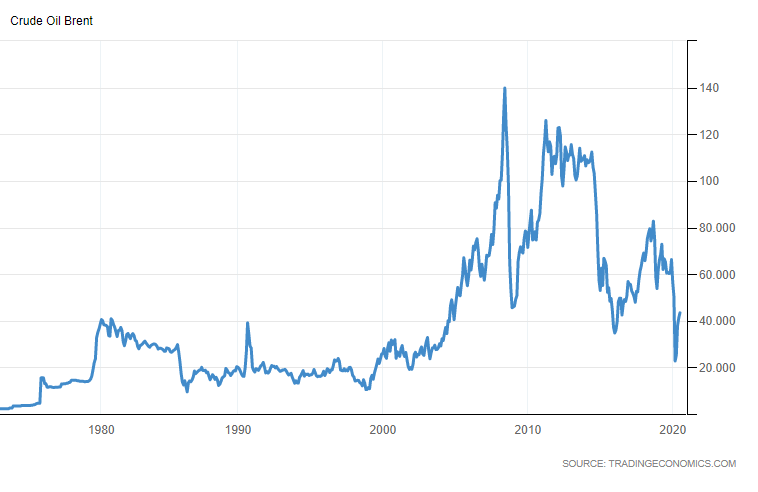
\includegraphics[width=12cm]{template_latex/Pictures/oil_brent.png}
    \caption{Oil price chart (\cite{brent})}
    \label{oilPrice}
\end{figure}

Before the establishment of OPEC in 1960, the oil price was monopolized by the western countries. After 1960, OPEC continuously struggled with Western multinational companies around the production and pricing power of oil.

In 1970s, with a series of victories of OPEC in negotiations, OPEC started to gain the power of the decision of the crude oil price. And the price started to rise at this period. The fourth Middle East war broke out in 1973 and resulted in the price increasing approximately 400\% to \$11 per barrel and the first energy crisis in Western countries. In February 1974, Nixon proposed to hold a meeting between oil-consuming countries then the International Energy Agency (IEA) was established. Energy supply issues have become a priority concern for governments. At the same time, the first modeling project leaded by U.S. government was created. Then a algorithm called "Project Independence Evaluation System (PIES)" (\cite{hogan1975energy}), and it was used for analysts to predict and develop strategies. From 1974 to 1978, crude oil prices remained at 
a certain level of \$11-\$14 per barrel. From 1979 to 1981, the second oil crisis doubled the oil price to the maximum price \$40 per barrel. These two crisis provided motivations for researchers to explore the oil market and subsequently a large amount of oil models were developed. The rising of OPEC's position changed the oil market structure as well as a lot of structural theories related with OPEC were also proposed in researchers' study. 
Later OPEC used the production quota in this period, the price of Brent oil fell slowly from US\$36.83 per barrel to US\$27.51 per barrel.
Then with the growth of crude oil production in non-OPEC oil-producing countries, the development of energy conservation technology and alternative energy sources. OPEC's ability to control oil prices had continued to decline, along with the fall of crude oil prices. In 1986, oil prices fell sharply to around \$10 per barrel. Subsequently the market power started to affect the oil price remains at a level of \$14.3-\$20 per barrel until 1997 except the short-term increase caused by the Gulf War between 1990 and 1991. As a result of the Asian financial crisis, demand decrease, and OPEC's untimely increase in production, the oil price dropped to around \$10 per barrel in 1998. 

Since then the price started to bounce and tripped the price in 18 months and continued to rise after 2003. The financial market began to gradually reflect its role in influencing short-term oil prices (\cite{huntington2013oil}). After reaching the nearly \$140 per barrel in 2008, the price fell sharply to \$45 at the end of the year with the broke out of the global financial crisis. From 2014-2016, the revolution of shale oil shocked the crude oil market. OPEC refused to reduce the production for defending the market share. From June 2014 to January 2016, the price of Brent crude oil fell from the \$115.06 to \$34 per barrel. The trade dispute between China and the United States in 2018 caused the price to fell from the highest price of \$82 to around \$53 per barrel. And then the Coronavirus in 2019 caused the reduction of the demand, with the oil price war between Russian and Saudi-Arabia in 2020 caused the Brent oil price to continue to drop in Spring 2020. The lowest price is \$22 on April 20, even the West Texas Intermediate (WTI) appeared negative price as the reason for that most May 2020 WTI oil futures contract holders could not store the oil as the contract was going to expired.

In recent years, the great development of the computer and the mathematical technology enables researchers to develop modeling systems with massive computing ability. Meanwhile, more historical and reliable data source are accessible. So more and more oil market models were generated compared with the past.
